\section{Reference experiments}\label{sec:numerics}

All experiments use externally specified Hamiltonians, so that remapping errors are isolated. The code is in
\texttt{prototype/} (Python/NumPy); every number in the tables below is generated from the files in
\texttt{results/} by \texttt{prototype/make\_tables.py}. Closed-form statements of
\cref{sec:continuum,sec:ot,sec:discrete,sec:structure} are checked by \texttt{prototype/verify\_propositions.py}
(11 checks, all passing: \cref{lem:edge}, \cref{prop:flux} and its example, the symbol \eqref{eq:symbol}, the kernel
dimensions of \cref{tab:rigidity}, \eqref{eq:cos2}, \cref{lem:lebesgue}, \cref{thm:ac}(iv), the $O(h^5)$ edge action
of quadratic elements, the curl of \cref{rem:force}, \cref{obs:vn}).

\paragraph{The oracle.} For a label $q$ the exact discrete transport $F^{\Delta t}_n(q)$, its action and its tangent
are obtained by integrating from the initial condition with the same integrator and step sequence. All errors are
measured against it, at the labels of the method under test; time-integration error cancels identically. The
\emph{non-adaptive reference} is the fixed Lagrangian mesh ($q_i$ uniform, never remapped), whose vertices are
exact oracle samples; its error is pure representation error.

\subsection{Two-dimensional phase space}\label{sec:num1d}

\paragraph{Setup.} $\X=\R/2\pi\Z$, $\mu=\dd q/2\pi$, kick--drift--kick with fixed $\Delta t$, initial sheet
$x_0=q$, $p_0=u_0+A\sin q$ ($\Sigma_0=u_0q-A\cos q$, $c=2\pi u_0$). Four tests:
\emph{twist} ($H=p^2/2-\cos x$, $u_0=2.6$, $A=0.5$: the sheet lies in the circulating region and phase-mixes
smoothly, developing many folds; $t\le40$);
\emph{collapse} (same $H$, $u_0=0.05$, $A=0$: a cold sheet falling into the pendulum well, crossing the separatrix; $t\le12$);
\emph{driven} ($H=p^2/2-\cos x-0.25\cos(x-1.7t)$, $u_0=0$, $A=0.3$: explicitly time dependent with a chaotic layer; $t\le12$);
\emph{comoving} ($H=p^2/2a(t)^2-0.25\cos x$, $a=t^{2/3}$, $t\in[1,40]$: the Einstein--de~Sitter form of \cref{sec:cosmo} with a prescribed potential).
Reconstructions: linear, cubic and quintic Lagrange interpolation in the label (orders 2, 4, 6), and the
action-corrected AC$(2,1)$, AC$(4,1)$, AC$(6,1)$ of \cref{thm:ac}. Sampling: \emph{fixed} or \emph{adaptive}; the
adaptive runs remap on a fixed schedule with the monitor
$M=\hat M_{\rm aff}+0.2+0.3\hat M_{\rm arc}+0.3\hat M_{\rm turn}$ (unit-mean normalised equi-affine, arclength and
turning-angle densities), the \emph{same} for all reconstructions, and the monotone-rearrangement map of \cref{prop:ot1d}.
So that the mesh sequence does not depend on whether a method carries the action, the reported runs evaluate
$\kappa$ in $\hat M_{\rm aff}=\abs\kappa^{1/3}$ from inscribed-triangle areas (also a symplectic invariant); driving the
monitor by the measured edge defects \eqref{eq:edgedefect} instead gives equivalent results for AC$(4,1)$
($e_\perp^{\max}=4.1\times10^{-6}$ against $4.3\times10^{-6}$ in the collapse test, $3.1\times10^{-6}$ against
$2.6\times10^{-6}$ in the driven test; \texttt{results/exp1d\_monitor\_ablation.json}).
Diagnostics: $e_\perp^{\max}$, $e_\parallel^{\max}$, the maximal normal and tangential distance between the
method's reconstruction and the oracle at four sub-sample labels per cell; the Poincar\'e invariant
$\oint p\,\dd x$ of the method's own carrier, by Gauss quadrature of the piecewise polynomial; total mass; energy
of the carrier against the oracle.

\begin{figure}[t]\centering
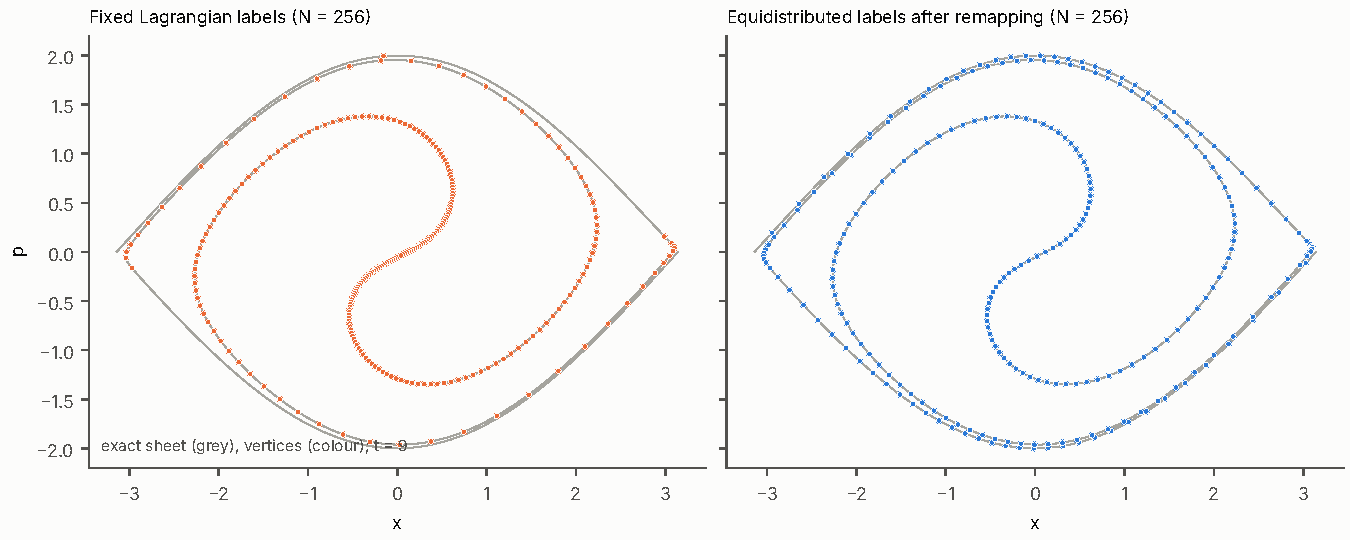
\includegraphics[width=0.86\textwidth]{../results/figures/fig_sheet.pdf}
\caption{Collapse test at $t=9$, $N=256$ vertices. Left: fixed Lagrangian labels leave the stretched outer
windings (labels near the stable manifold of the hyperbolic point) essentially unsampled. Right: labels after
optimal-transport remapping with the AC$(4,1)$ reconstruction. The label density varies by several orders of
magnitude; the mass per cell varies accordingly (\cref{prop:sampling}).}\label{fig:sheet}
\end{figure}

\begin{figure}[t]\centering
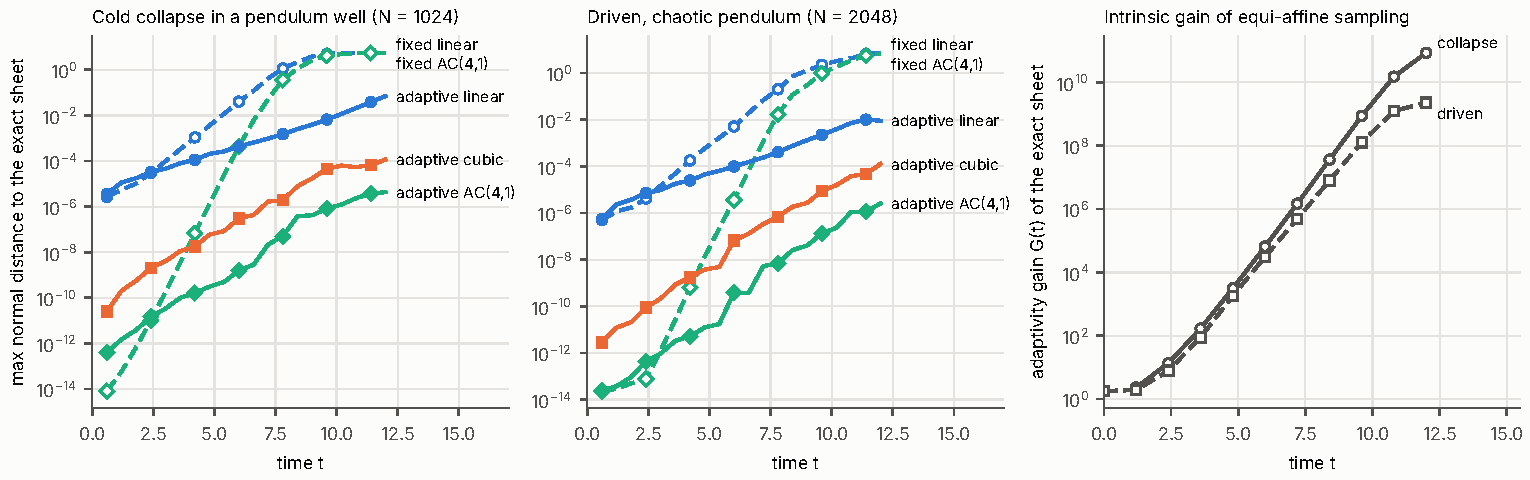
\includegraphics[width=\textwidth]{../results/figures/fig_history.pdf}
\caption{Normal error against the exact sheet for the collapse and driven tests (left, centre), and the
adaptivity gain $G(t)$ of \eqref{eq:complexity} for the exact sheets (right). Fixed sampling fails when $G$
becomes large, whatever the reconstruction; adaptive sampling with the action-corrected remap retains
$10^{-6}$.}\label{fig:history}
\end{figure}

\begin{table}[t]\centering\footnotesize
\resizebox{\textwidth}{!}{\TableHistory}
\caption{Final-time diagnostics, all tests ($c$: exact Liouville class; $E$: oracle energy). The total-mass error
is $0$ in every run (not shown). Remaps every 50, 20, 20, 25 steps respectively.}\label{tab:history}
\end{table}

\paragraph{Results.}
\emph{(1) Exact invariants.} For every action-corrected reconstruction the Poincar\'e invariant of the carrier
equals $c$ to round-off ($\le6\times10^{-15}$ absolute, with $c$ up to $16.3$) in all tests, for all $N$, and for
1 to 399 remaps (\cref{tab:history,tab:conv,tab:accum}), including the explicitly time-dependent Hamiltonians, as
\cref{thm:scheme}(ii) asserts. The interpolation remaps drift: linear by up to $-0.37$, cubic by up to
$3.8\times10^{-4}$, quintic by $6.7\times10^{-6}$ at 399 remaps, growing with the number of remaps as predicted by
\cref{thm:budget}; linear interpolation loses action monotonically (\cref{cex:polygon}).

\emph{(2) Accuracy.} On exact samples (fixed rows of \cref{tab:conv}) AC$(4,1)$ converges at order $5.00$ in the
normal direction against $4.00$ for the cubic it corrects, with tangential order 4 unchanged, confirming
\cref{thm:ac}(iii). With 39 remaps the adaptive AC$(4,1)$ run converges at order $\simeq4.6$ and is two to three
orders of magnitude more accurate than cubic remapping at equal $N$; AC$(6,1)$ reaches the round-off conditioning
floor of \cref{rem:roundoff} ($\sim10^{-9}$ at $N=4096$).

\emph{(3) Accumulation.} For AC$(4,1)$ the final normal error varies only between $1.7\times10^{-7}$ and
$9.4\times10^{-7}$ as the number of remaps goes from 1 to 399 (\cref{tab:accum}); the cubic remap degrades from
$2\times10^{-5}$ to $4.5\times10^{-4}$ and the linear one is destroyed. No instability is observed
(cf.\ \cref{obs:vn}).

\emph{(4) When adaptivity matters.} In the twist test the exact sheet has $G(t)\le21$: uniform labels are nearly
optimal and remapping buys nothing; with the same reconstruction the fixed mesh is more accurate than the
remapped one (\cref{tab:history}). This is an honest negative result for adaptivity on smooth phase mixing. In
the collapse and driven tests $G$ grows exponentially (\cref{tab:complexity}), reaching $10^{9}$--$10^{11}$ at
$t=12$, and the fixed mesh has normal error above $0.1$ from $t\approx7$--$8$ and $O(1)$ at the end for \emph{every} reconstruction, while the adaptive
action-corrected runs retain $e_\perp^{\max}=4\times10^{-6}$ ($N=1024$) and $3\times10^{-6}$ ($N=2048$). The smallest
label spacing produced by the remap at $t=12$ is $1.2\times10^{-6}$ against $6\times10^{-3}$ for uniform labels: a
fixed mesh would need several thousand times more vertices.

\emph{(5) Tangential error and mass.} The tangential error, which is the error in the \emph{placement of mass along
the sheet}, is not improved by the action (it is $O(h^m)$ for both families) and is the dominant error of the
action-corrected schemes ($3\times10^{-3}$ in the collapse test, concentrated where the sheet is exponentially
stretched and carries little mass; the mass-weighted $L^2$ normal error there is $10^{-7}$). Total mass is exact.

\emph{(6) A failure that taught something.} The first front implementation (parabolic arc as a graph over the
chord with a metric normal, tangential map by cubic interpolation; superseded and not retained in the repository) preserved the invariant exactly but converged
erratically; the maximal error sat at hairpin turns, where the phase-space speed $\abs{F'}$ is small and the
chord frame rotates by $O(1)$ between cells. The parametric form \eqref{eq:ac}, which commutes with affine symplectic
maps up to a higher-order term, removed the problem. We record it because it shows that \emph{exact invariants do
not imply accuracy}, and that equivariance under the affine symplectic group is a genuine design constraint.

\begin{figure}[t]\centering
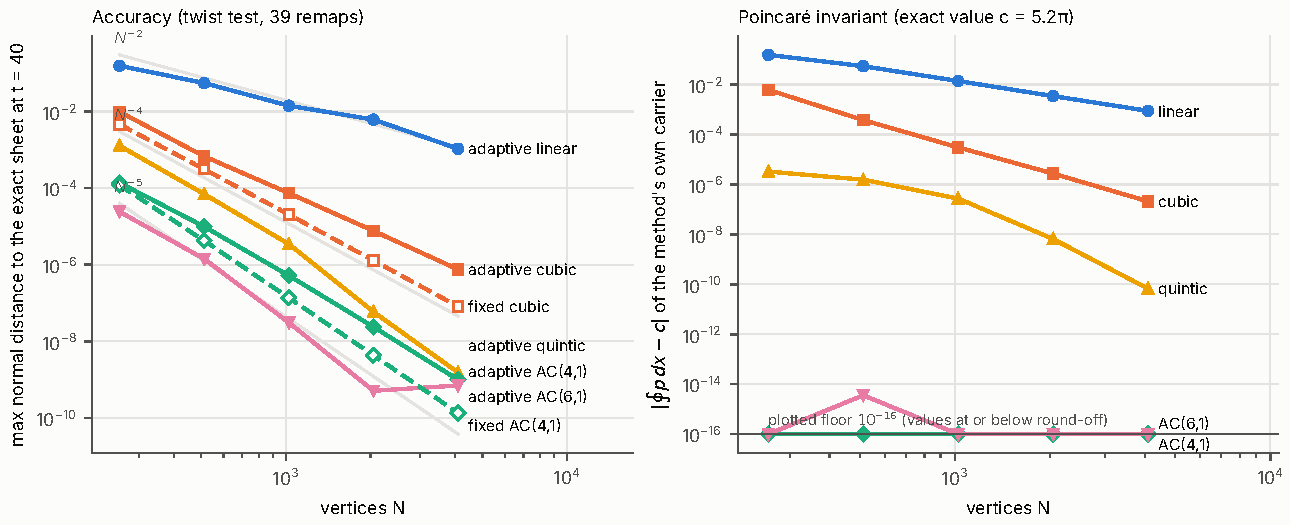
\includegraphics[width=0.92\textwidth]{../results/figures/fig_convergence.pdf}
\caption{Twist test, $t=40$, 39 remaps. Left: normal error versus $N$ (dashed: fixed Lagrangian mesh with the
same reconstruction). Right: error of the Poincar\'e invariant of each method's carrier; the action-corrected
schemes are at round-off (plotted at a floor).}\label{fig:conv}
\end{figure}

\begin{table}[t]\centering\footnotesize
\resizebox{\textwidth}{!}{\TableConvergence}
\caption{Twist test, $t=40$, 39 remaps (adaptive rows): $e_\perp^{\max}$ and observed order between the last two
resolutions (for AC$(6,1)$, between $N=1024$ and $2048$, the $N=4096$ value being at the conditioning floor).}\label{tab:conv}
\end{table}

\begin{figure}[t]\centering
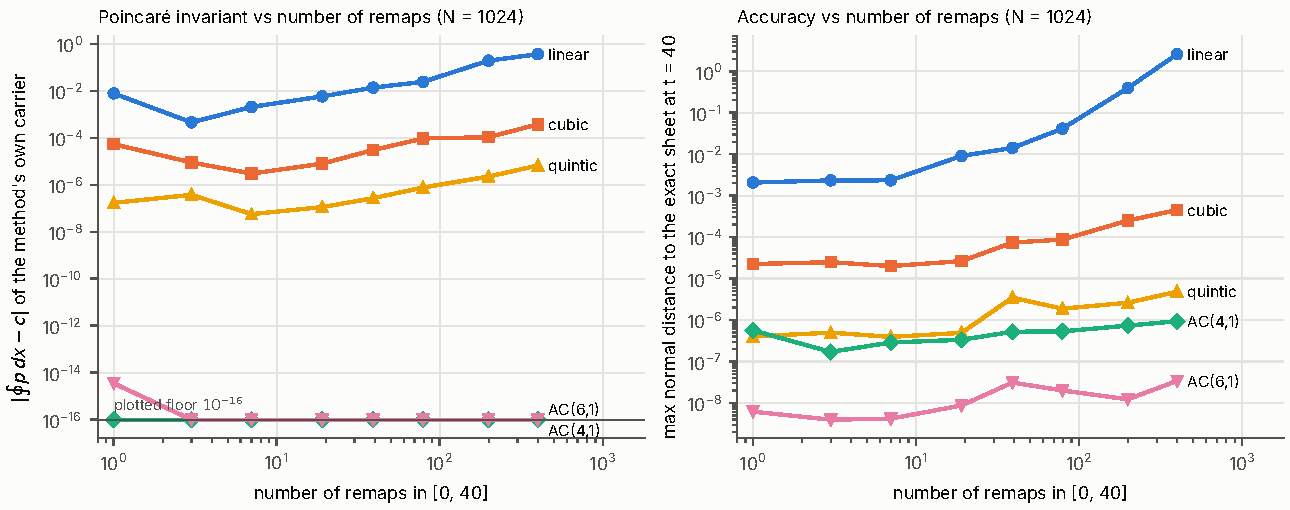
\includegraphics[width=0.92\textwidth]{../results/figures/fig_accumulation.pdf}
\caption{Twist test, $N=1024$: Poincar\'e invariant error and normal error at $t=40$ as functions of the number of
remaps.}\label{fig:accum}
\end{figure}

\begin{table}[t]\centering\scriptsize
\resizebox{\textwidth}{!}{\TableAccumulation}
\caption{Twist test, $N=1024$, $t=40$: dependence on the number of remaps.}\label{tab:accum}
\end{table}

\begin{table}[t]\centering\footnotesize
\TableComplexity
\caption{Intrinsic complexity of the exact sheets (oracle, $2^{16}$ labels): equi-affine length $\mathcal A$,
Euclidean length, maximal affine curvature and adaptivity gain $G$ of \eqref{eq:complexity}.}\label{tab:complexity}
\end{table}

\subsection{Four-dimensional phase space, single-stream regime}\label{sec:num2d}

\paragraph{Setup.} $\X=\T^2$, $H=\abs p^2/2+V(x)$,
$V=-(2\pi)^{-2}[\cos2\pi x_1+\cos2\pi x_2+\tfrac12\cos2\pi(x_1-x_2)]$, cold initial sheet $x=q$, $p=0$, $\Sigma=0$
($c=0$), $\Delta t=0.01$, $t\le0.9$ (linearised estimates: first shell crossing at $t\simeq1.11$, minimal $\det D_qx\simeq0.18$ at the end).
Reference grid $n\times n$, $n=32,64,128$. Remaps at steps 30, 50, 70: monitor
$M\propto(\norm C^2+(0.15\langle\norm C\rangle)^2)^{1/5}$ from the cubic form \eqref{eq:cubic}, mollified with a
Gaussian of label-space width $0.05$; Monge--Amp\`ere solve for $\varphi$; point location through the spectral
label map $\id+\nabla\varphi$. Reconstructions: bilinear, bicubic and biquintic splines of $(x,p)$ in $\xi$, and the
generating-function elements of \cref{thm:front} in the identity frame, \emph{front-3} ($x$: bicubic spline, $W$:
$C^1$ bicubic Hermite) and \emph{front-5} ($x$: biquintic spline, $W$: $C^2$ biquintic Hermite), with exact nodal
values and gradients \eqref{eq:hermitedata} and higher nodal derivatives from sixth-order differences of the gradient
data. Diagnostics: momentum error against the oracle at the nodes; circulation $\oint p_h\cdot\dd x_h$ of each
method's carrier along the images of 24 fixed circles in $\Xi$ (exact value $0$), by Richardson-extrapolated
trapezoid quadrature on 4096/8192 chords; total mass from the label cells.

\begin{figure}[t]\centering
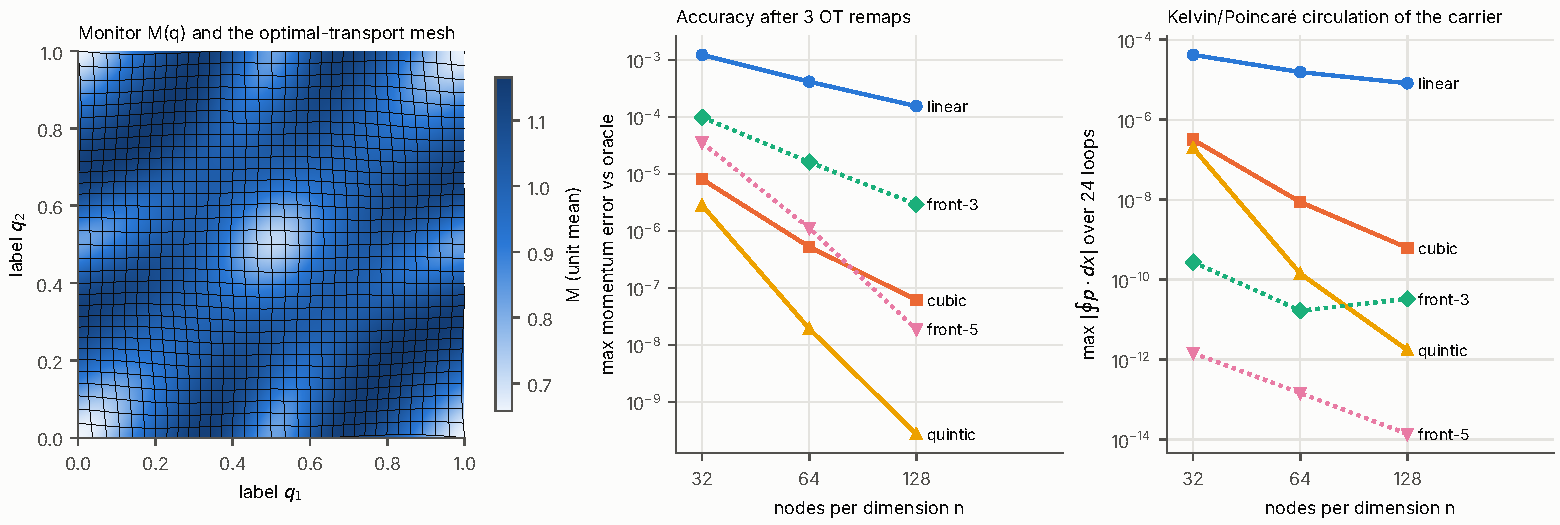
\includegraphics[width=\textwidth]{../results/figures/fig_2d.pdf}
\caption{$d=2$. Left: monitor on label space and the image of the reference grid under the optimal-transport map
($n=64$, every second line). Centre: momentum error after three remaps. Right: maximal circulation of each
carrier.}\label{fig:2d}
\end{figure}

\begin{table}[t]\centering\footnotesize
\resizebox{\textwidth}{!}{\TableTwoD}
\caption{$d=2$, $t=0.9$. Total-mass error $\le$\TwoDMassErr\ in all runs; cell masses vary by a factor up to
\TwoDMassRatio.}\label{tab:2d}
\end{table}

\begin{table}[t]\centering\footnotesize
\resizebox{\textwidth}{!}{\TableOT}
\caption{Monge--Amp\`ere solves of the front-5 run at $n=128$.}\label{tab:ot}
\end{table}

\paragraph{Results.}
\emph{Optimal transport.} The Newton--Krylov solver converges in 4--5 iterations to residual $10^{-13}$, with
$\lambda_{\min}(I+D^2\varphi)\ge0.86$ (\cref{tab:ot}); in a stand-alone test with monitor contrast $148$ it converged
in 6 iterations with $\lambda_{\min}=0.37$. The total mass computed from the label cells equals one to round-off
while individual cell masses vary (\cref{prop:mass,prop:sampling}).

\emph{Structure.} The carriers of the generating-function elements have circulation at the level of the loop
quadrature ($10^{-12}$--$10^{-14}$ for front-5; $10^{-11}$--$10^{-10}$ for front-3, whose momentum is only $C^0$ across cells,
which limits the extrapolated quadrature, not the identity $p_h\cdot\dd x_h=\dd W_h$). The spline carriers have a
genuine defect: $4\times10^{-5}\to8\times10^{-6}$ (bilinear), $3\times10^{-7}\to6\times10^{-10}$ (bicubic),
$2\times10^{-7}\to2\times10^{-12}$ (biquintic) for $n=32\to128$, larger than for the same reconstructions on exact
data (lower block of \cref{tab:2d}), i.e.\ created by the remaps.

\emph{Accuracy.} After three remaps the observed orders of the momentum error between successive resolutions are
$2.6,\,2.5$ for front-3 (third order on exact data) and $5.0,\,5.9$ for front-5, consistent with
\cref{thm:front}(iv); the plain splines of the same degree are about one order \emph{more} accurate in $p$
(bicubic: $3.9,\,3.1$; biquintic: $7.2,\,6.1$), because they interpolate $p$ directly whereas the front element
differentiates $W$. Thus in $d\ge2$, with the elements tested, exact Lagrangian structure costs one order of
momentum accuracy relative to an unconstrained spline of the same degree, in contrast to $d=1$ where the action
\emph{gains} one order. Since the monitor contrast is small here ($\le1.8$), adaptivity brings no accuracy gain in this
regime; the experiment demonstrates the mechanics and the structure, not a pay-off.

\emph{Monitor regularity.} With a non-smooth monitor ($\norm C$ with a mesh-scale smoother) and a bicubic label
map the remap errors of all higher-order reconstructions degraded to first order; \cref{rem:monreg} records the
remedy used above.

\paragraph{Limitations of the experimental evidence.} No self-consistent force; no multi-stream test in $d=2$
(the chart-wise element is singular at caustics, \cref{prob:glue}); no $d=3$ run; schedules rather than
error-controlled triggers; one family of monitors.
